\newcommand{\decktitle}{Python IV - Weitere Themen}

%%%%%%%%%%%%%%%%%%%%%%%%%%%%%%%%%%%%%%%%%%%%%%%%%
%
% DOCUMENT
%
%%%%%%%%%%%%%%%%%%%%%%%%%%%%%%%%%%%%%%%%%%%%%%%%%

\begin{frame}
    \subtitle{\decktitle}
    \titlepage
\end{frame}


\begin{frame}
    \frametitle{\textbf{Outline:}}
    \tableofcontents
\end{frame}

		
\section{Exceptions}

    \begin{frame}{Exceptions (I)}
        Manchmal treten bei der Programmierung unvorhergesehene Fehler auf. Dies passiert häufig während der Entwicklung eines Programms und kann somit einfach behoben werden. Befindet sich eine Software jedoch im Produktivbetrieb, kann ein unvorhergesehener Fehler unter Umständen zu weitreichenden und schwerwiegenden Konsequenzen führen. \\~\
        
        Daher sollte bereits während der Planung und Entwicklung eines Programms auf die Qualität und Fehlerfreiheit geachtet werden.
    \end{frame}
    
    \begin{frame}{Exceptions (II)}
        Sollte während der Ausführung eines Programms ein Fehler auftreten, so wird vom Python Interpreter automatisch eine sogenannte \textbf{Exception} erzeugt. \\~\
        
        Der Name \textit{Exception} kommt daher, dass im Falle eines Fehlers eine Ausnahmebehandlung durchgeführt werden kann. Das bedeutet, dass der Fehler beispielsweise im weiteren Verlauf des Programms behoben werden kann (siehe Exeption-Handling). \\~\
        
        Ohne das sogenannte "Abfangen" einer Exception führt eine Exception grundsätzlich zum Abbruch des Programms. Der Grund hierfür ist, dass der Python Interpreter nicht weiß, wie mit einem möglichen Fehler umgegangen werden soll und da sich das Programm nicht in einem undefinierten Zustand befinden kann, wird es beendet.
    \end{frame}
    
    \begin{frame}[fragile]{Exceptions (III)}
        Sollte aus irgendeinem Grund eine Exception erzeugt werden, wird mithilfe des sogenannten \textbf{Stack-Traces} angezeigt
        \begin{enumerate}
            \item was der Grund des Fehlers ist
            \item wo der Fehler aufgetreten ist
            \item was den Fehler ausgelöst hat
        \end{enumerate}
        
        \\~\
        
        Dies kann am einfachsten durch die folgenden Beispiele dargestellt werden:
        
    \end{frame}
    
    \begin{frame}[fragile]{Exceptions (IV)}
\begin{exampleblock}{Beispiel 1: Division durch 0}
\begin{pyconcode}
>>> 1/0
Traceback (most recent call last):
  File "<stdin>", line 1, in <module>
ZeroDivisionError: division by zero
\end{pyconcode}            

Hier wurde der Fehler durch eine Division mit 0 ausgelöst. Daher wird ein \textbf{ZeroDivisionError} erzeugt ("geworfen").
\end{exampleblock}
    \end{frame}
    
    \begin{frame}[fragile,allowframebreaks]{Exceptions (V)}
\begin{exampleblock}{Beispiel 2: Datei nicht gefunden}
\begin{pythoncode}
def open_file(filename):
    open(filename)


if __name__ == "__main__":
    open_file("test.txt")
\end{pythoncode}
\begin{pyconcode}
Traceback (most recent call last):
  File "exception.py", line 6, in <module>
    open_file("test.txt")
  File "exception.py", line 2, in open_file
    open(filename)
FileNotFoundError: [Errno 2] No such file or directory: 'test.txt'
\end{pyconcode}            

\end{exampleblock}
\begin{exampleblock}

Hier wurde der Fehler ausgelöst, indem eine Datei namens "test.txt" geöffnet werden soll, die aber im aktuellen Verzeichnis nicht existiert. Daher wird ein \textbf{FileNotFoundError} geworfen. \\~\

Wird der Code direkt über die Kommandozeile eingegeben (wie im 1. Beispiel), tritt der Fehler unmittelbar nach der Eingabe bzw. Ausführung der problematischen Anweisung auf und kann daher leicht lokalisiert werden. Wird der Code jedoch über den Inhalt einer oder mehrerer Dateien ausgeführt, die mitunter hunderte Zeilen besitzen können, fällt es schwerer, den Fehler genau zu lokalisieren, da der Fehler erst bei einer Ausführung des gesamten Programms auftritt und nicht direkt bei der Eingabe des jeweiligen Befehls. \\~\

Daher bietet der Stack-Trace zusätzliche Informationen, wo genau der Fehler aufgetreten ist. Im obigen Beispiel ist etwa zu erkennen, dass der Fehler in Zeile 2 der Datei \code{exception.py} aufgetreten ist. Dieser Aufruf wurde wiederum durch einen Aufruf in Zeile 6 der selbigen Datei ausgelöst. Mithilfe des Stack-Traces kann also genau zurückverfolgt werden, wo der Fehler auftritt und welche Funktionsaufrufe diesen ausgelöst haben.
\end{exampleblock}
    
    \end{frame}
    
    \begin{frame}[fragile,allowframebreaks]{Exceptions (VI)}
        
        \begin{exampleblock}{Beispiel 3: String-/Integer Konkatenation}
\begin{pythoncode}
def get_user_info():
	name = input("Wie heißt du?: ")
	age = int(input("Wie alt bist du?: "))

	return name, age

def print_user_info():
	name, age = get_user_info()
	print("Hallo " + name + ", du bist " + age + " Jahre alt." )

if __name__ == "__main__":
	print_user_info()
\end{pythoncode}
\end{exampleblock}

\vbox{
\begin{exampleblock}{Beispiel 3: String-/Integer Konkatenation}
\begin{pyconcode}
"Wie heißt du?: Jonas"
"Wie alt bist du?: 27"
Traceback (most recent call last):
  File "test.py", line 12, in <module>
    print_user_info()
  File "test.py", line 9, in print_user_info
    print("Hallo " + name + ", du bist " + age + " Jahre alt." )
TypeError: can only concatenate str (not "int") to str
\end{pyconcode}            
\end{exampleblock}
}

    \end{frame}
    
    \begin{frame}[fragile]{Exception Handling (I)}
        Da im Falle einer auftretenden Exception die Ausführung des Programms ohne weitere Maßnahmen des Programmierers grundsätzlich abgebrochen wird, stellen diese Fehler häufig ein unerwünschtes Verhalten dar, da die Software im Produktivbetrieb möglichst fehlerfrei und stabil laufen sollte.\\~\ 
        Dennoch können auftretende Exceptions meist nicht vollständig vermieden werden, insbesondere bei der Verarbeitung von Daten, die während der Entwicklung noch nicht bekannt sind, sondern erst während der Ausführung des Programms eingelesen werden (z.B. durch Nutzereingaben, Datenbankabfragen, ...).\\~\
        Da diese Daten zunächst nicht bekannt sind, muss sich der Entwickler überlegen, welche Fehler bei der späteren Verarbeitung der Daten potentiell auftreten könnten, z.B. Speicherort der Daten existiert nicht, Umwandlung von Datentypen schlägt fehl, mathematisch ungültige Rechenoperationen, etc.
    \end{frame}
    
    \begin{frame}[fragile]{Exception Handling (II)}
        Der Programmierer muss sich bereits während der Entwicklung des Programms um diese möglicherweise auftretenden Fehler kümmern, sodass diese nicht unmittelbar zu einem Absturz des Programms führen. Falls also eine Exception auftreten sollte, muss der Programmierer definieren, was stattdessen passieren soll. Dieses Vorgehen wird als \textbf{Exception Handling} bezeichnet.
    \end{frame}
    
    \begin{frame}[fragile]{Exception Handling (III)}
        Das Exception Handling besteht immmer aus mindestens 2 Teilen:
        \begin{enumerate}
            \item Zunächst wird angegeben, welche Funktion das Programm ausführen soll. Dies ist die Stelle, an der die Exception auftreten kann (\textbf{try}-Block)
            \item Code, der ausgeführt wird, falls die Exception auftritt. Da sich das Programm nicht in einem undefinierten Zustand befinden kann, muss der Programmierer angeben, was stattdessen passieren soll (\textbf{except}-Block)
        \end{enumerate}\\~\
        
        Das Exception Handling wird immer mit den Schlüsselwörtern \code{try} und \code{except} beschrieben.
    \end{frame}
    
    \begin{frame}[fragile]{Exception Handling (IV)}

    
\begin{exampleblock}{Beispiel: Division}
In folgendem Beispiel werden 2 Zahlen vom Nutzer eingelesen, dividiert und das Ergebnis schließlich ausgegeben.

\begin{pythoncode}
num_1 = float(input("Bitte 1. Zahl eingeben: "))
num_2 = float(input("Bitte 2. Zahl eingeben: "))

result = num_1 / num_2
print(f"Das Ergebnis der Division ist {result}")
\end{pythoncode}

Dieser Codeausschnitt ist problemlos ausführbar, solange der Nutzer für die Zahl \code{num\_2} eine Zahl ungleich 0 eingibt. Im Falle einer Division durch 0 wird ansonsten wie oben beschrieben ein \code{ZeroDivisionError} geworfen.\\~\

Diese Problematik muss der Programmierer bereits während der Entwicklung erkennen und eine entsprechende Fehlerbehandlung bereitstellen, falls der Nutzer tatsächlich die Zahl 0 eingeben sollte.
\end{exampleblock}    

    \end{frame}
    
    \begin{frame}[fragile,allowframebreaks]{Exception Handling (V)}
\begin{pythoncode}
num_1 = float(input("Bitte 1. Zahl eingeben: "))
num_2 = float(input("Bitte 2. Zahl eingeben: "))

try:
    result = num_1 / num_2
    print(f"Das Ergebnis der Division ist {result}")
except ZeroDivisionError:
    print("Diese Berechnung ist nicht möglich, als 2. Zahl muss ein Wert != 0 eingegeben werden.")
\end{pythoncode}

In diesem Fall ist der "problematische" Code (\code{result = num\_1 / num\_2}) in einem \code{try}-Block enthalten. Es wird also zunächst versucht, den Code fehlerfrei auszuführen. Ist dies möglich, wird der \code{except}-Block übersprungen. Dieser wird lediglich dann ausgeführt, wenn im \code{try}-Block die entsprechende Exception auftritt, die abgefangen werden soll (in diesem Fall \code{ZeroDivisionError}).\\  \framebreak

Im Beispiel wird also das Ergebnis der Kalkulation ausgegeben, falls \code{num\_2} != 0, andernfalls wird der Nutzer aufgefordert, als 2. Zahl einen anderen Wert als 0 einzugeben.\\~\

Dies bietet also den Vorteil, mögliche Fehler abzufangen und zu behandeln, anstatt das Programm zum Absturz zu führen.

    \end{frame}
    
    \begin{frame}[fragile]{Exception Handling - Beispiel aus der Realität (I)}
Warum ist Exception Handling so wichtig?\\~\

Beispiele aus der Realität zeigen, dass Exception Handling enorm wichtig ist, um ungewollte oder unerwartete Funktionsausfälle zu vermeiden. \\~\

Ein System, in dem ein auftretender Fehler nicht korrekt behandelt wird, kann schwerwiegende finanzielle, technische oder auch soziale Folgen haben.
    \end{frame}
    
    \begin{frame}[fragile]{Exception Handling - Beispiel aus der Realität (II))}
Ein gutes Beispiel für fehlendes Exception Handling, was letztendlich schwerwiegende Konsequenzen mit sich brachte, ist der Flug 88 der europäischen Schwerlast-Trägerrakete \textbf{Ariane 5}.\\~\

Am 04.Juni 1996 sollte die neu konstruierte Ariane 5 Rakete erstmals starten, mit der in Zukunft Kommunikationssatelliten transportiert und Starts der Hermes-Raumfähre ermöglicht werden sollten.\\~\

Für die Trägerrakete sollte eine Zuverlässigkeit von 98-99\% erreicht werden, die maximal akzeptable Anzahl an Fehlstarten liegt demnach bei 1 bzw. 2 bei 100 Starts \cite{AAIA}.
    \end{frame}
    
    \begin{frame}[fragile]{Exception Handling - Beispiel aus der Realität (III))}
    
    
    \begin{minipage}{\textwidth}
\begin{columns}[T]
\begin{column}{0.5\textwidth}
\begin{figure}
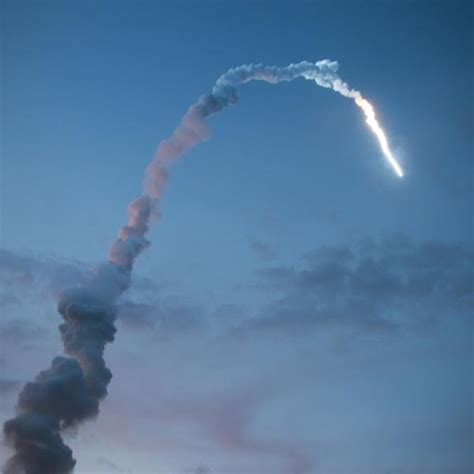
\includegraphics[keepaspectratio, width=0.9\linewidth]{chapters/10_python4_further_topics/figures/ariane.jpeg}
\caption{Die Explosion von Ariane 5 39 Sekunden nach dem Start}
\end{figure} 
\end{column}
\begin{column}{0.5\textwidth}
Etwa 39 Sekunden nach dem Start kam die Rakete von ihrem vorgegebenen Kurs ab, brach auseinander und sprengte sich in der Folge selbst.\\~\

Die Entwicklungskosten der Ariane 5 lagen bei etwa 5,8 Milliarden Euro, der materielle Schaden von Rakete und Nutzlast lag bei etwa 290 Millionen Euro \cite{arianefailure}. Der wirtschaftliche Gesamtschaden dürfte aber deutlich größer sein, da durch diesen Unfall die komplette Entwicklung der Raketen komplett neu gestartet wurde, was zu enormen Verzögerungen führte. Bis ins Jahr 2003 wurden daraufhin primär die Vorgängermodelle Ariane 4 eingesetzt.

\end{column}
\end{columns}
\end{minipage}



    \end{frame}
    
    \begin{frame}[fragile]{Exception Handling - Beispiel aus der Realität (IV))}
     \textbf{Was war passiert?} \\~\
     
     Mithilfe des Trägheitsnavigationssystems wird die horizontale Ausrichtung (\textit{"horizontal bias"}) des Flugkörpers bestimmt, also ob die Rakete nach oben oder nach unten zeigt. \\~\
     Dieser Wert wurde in einer 64-Bit Variable gespeichert (Anzahl möglicher Werte: $2^{64}$), anschließend jedoch in eine 16-Bit Variable umgewandelt (Anzahl möglicher Werte: $2^{16}$ = 65.536). In den ersten Sekunden des Flugs war die Beschleunigung der Rakete eher gering, wodurch eine Umwandlung problemlos funktionierte. Erst als die Beschleunigung immer höher wurde, konnte die Zahl in der 64-Bit Variablen nicht mehr ohne Datenverlust in die 32-Bit Variable umgewandelt werden. Anders als in Python ist bei Ada, der damals verwendeten Programmiersprache, eine Umwandlung mit Datenverlust nicht ohne weiteres möglich, sodass dies zu einem \textit{arithmetischen Überlauf} führte.
    \end{frame}
    
    \begin{frame}[fragile]{Exception Handling - Beispiel aus der Realität (V))}
     Dieser unbehandelte Fehler führte zum Ausfall des Reserve- und Hauptnavigationssystems, was wiederum dazu führte, dass Lenk- und Lageinformationen nicht mehr bestimmt werden konnten.\\~\
     Anstatt des eigentlichen Wertes war in der Variablen nun ein diagnostischer Wert gespeichert, welcher auf den aufgetretenen Fehler hinweisen sollte. Dieser Wert wurde aber vom Bordcomputer als normaler Flugwert interpretiert, wodurch eine große Abweichung von der vorgesehenen Flugbahn berechnet wurde. Die Düsen der Rakete wurden daraufhin auf eine Schwenkung von über 30 Grad pro Sekunde eingestellt, durch die starke Lufströmung aufgrund der noch dichteren Schichten in Erdnähe brachen die Düsen auseinander. In der Folge risssen die Verbindungen zwischen den Feststoffboostern und der Hauptstufe ab. Dies führte wie in einem solchen Fall vorgesehen zur Selbstzerstörung der Rakete.
    \end{frame}
    
    \begin{frame}[fragile]{Exception Handling - Beispiel aus der Realität (VI))}
     Ein solches Unglück aus der Realität zeigt also, welche Auswirkungen ein kleiner unbedeutend-scheinender Softwarefehler haben kann. \\~\
     Außerdem macht dieses Beispiel deutlich, wie wichtig in einem produktiven Umfeld Fehlerbehandlung und Software Tests sind. Zwar werden die wenigsten von uns an der Softwareentwicklung einer Rakete mitwirken, doch auch in vielen anderen Projekten ist das Schadenspotential groß.
    \end{frame}